% 通路分類モジュールの詳細図．paper.tex から \input して使う．
% 画像・BEV は未学習環境 m の実データおよび UniDepth の実出力．
% 各ブロックは隣のブロックからの間隔（\gap）で配置する．
\begin{tikzpicture}[
    font=\normalsize,
    blk/.style={draw, align=center, minimum height=8mm, minimum width=16mm,
                inner xsep=2pt},
    val/.style={draw, align=center, minimum height=6.5mm, minimum width=10mm},
    pic/.style={draw, inner sep=0pt},
    grp/.style={draw, dashed, gray},
    frz/.style={fill=cyan!12},
    lbl/.style={font=\small, inner sep=1.5pt},
    ar/.style={-{Latex[length=1.6mm]}, thin},
]
\def\gap{3mm}
% BEV 枝は UniDepth から 128-D までを等間隔にする（上段の幅から決めた値）．
\def\botgap{7.4mm}
% 各行の高さ
\coordinate (top) at (0,0);
\coordinate (mid) at (0,-1.8);
\coordinate (bot) at (0,-3.6);

% ---- 入力 ----------------------------------------------------------------
\node[pic] (rgb) at (0,-1.7) {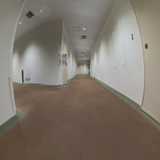
\includegraphics[width=13mm]{images/cc_rgb.png}};
\node[lbl, below=0.5mm of rgb] {RGB image};
\coordinate (rsplit) at ([xshift=2.5mm]rgb.east);

% ---- RGB 枝 --------------------------------------------------------------
\node[blk, anchor=west] (res) at ([xshift=\gap]rsplit |- top) {Resize\\$224\times224$};
\node[blk, frz, right=\gap of res] (dno) {\DINOvTwo\ ViT\text{-}S/14\\\small \frozen};
\node[blk, right=\gap of dno] (rdo) {Spatial readout\\\small CLS $+$ 3 regional means};
\node[val, right=\gap of rdo] (f15) {$1536$\text{-}D};
\node[pic] (b2) at (rdo |- 0,-1.4) {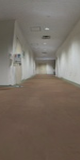
\includegraphics[width=6mm]{images/cc_band2.png}};
\node[pic] (b1) at ([xshift=-7mm]b2) {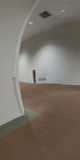
\includegraphics[width=6mm]{images/cc_band1.png}};
\node[pic] (b3) at ([xshift=7mm]b2) {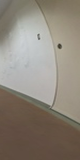
\includegraphics[width=6mm]{images/cc_band3.png}};
\node[lbl, below=0.5mm of b2] {left \,\textbar\, center \,\textbar\, right};

% ---- BEV 枝 --------------------------------------------------------------
\node[blk] (udp) at (res |- bot) {\UniDepth};
\node[pic, right=\botgap of udp] (dep) {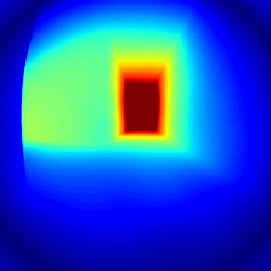
\includegraphics[width=11mm]{images/pf_depth_cmap.png}};
\node[pic, right=\botgap of dep] (bev) {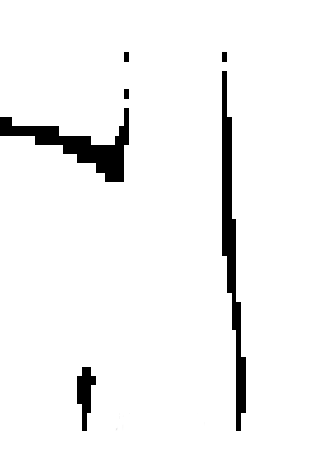
\includegraphics[height=15mm]{images/cc_bev_inner.png}};
\draw (bev.south west) rectangle (bev.north east);
\node[lbl, below=0.5mm of bev] {BEV $50\times70$};
\node[blk, right=\botgap of bev] (cnn) {BEV CNN\\\small $4\times4$ pooling};

% ---- 分類ヘッド ----------------------------------------------------------
% 1536-D と 128-D は Feature fusion の真上と真下に置き，縦の矢印で結ぶ．
\node[blk] (fus) at (f15 |- mid) {Feature fusion\\\small $256$\text{-}D};
\node[val] (f12) at (f15 |- bot) {$128$\text{-}D};
\node[blk, right=\gap of fus] (gru) {GRU\\\small 3 frames, stride 4};
\node[blk, right=\gap of gru] (lin) {Linear $+$\\sigmoid};
\node[val, minimum width=13mm, right=4mm of lin] (pr) {$p(\mathrm{right})$};
\node[val, minimum width=13mm, above=2.5mm of pr] (pf) {$p(\mathrm{front})$};
\node[val, minimum width=13mm, below=2.5mm of pr] (pl) {$p(\mathrm{left})$};

% ---- 結線 ----------------------------------------------------------------
\draw[thin] (rgb.east) -- (rsplit);
\draw[ar] (rsplit) |- (res.west);
\draw[ar] (rsplit) |- (udp.west);
\draw[ar] (res) -- (dno);
\draw[ar] (dno) -- (rdo);
\draw[ar] (rdo) -- (f15);
\draw[ar] (udp) -- (dep);
\draw[ar] (dep) -- (bev);
\draw[ar] (bev) -- (cnn);
\draw[ar] (cnn) -- (f12);
\draw[ar] (f15) -- (fus);
\draw[ar] (f12) -- (fus);
\draw[ar] (fus) -- (gru);
\draw[ar] (gru) -- (lin);
\draw[ar] (lin.east) -- (pf.west);
\draw[ar] (lin.east) -- (pl.west);
\draw[ar] (lin.east) -- (pr.west);

\end{tikzpicture}
